%% Department of Biostatistics Consulting Report Template
%% Version 2.2
%% Sarah R Haile, 2010.12.14
%% Sina Rüeger, 2012.02.20, 2012.12.06 (for STA490)
%% Eva Furrer, 2013.02.01 (for STA490)
%% Isaac Gravestock, 2014.09.01 (Update for RStudio, knitr)
%% Verena Steffen, 2016.05.30 (for STA490)
\documentclass[11pt,a4paper,twoside]{article}\usepackage[]{graphicx}\usepackage[]{color}
%% maxwidth is the original width if it is less than linewidth
%% otherwise use linewidth (to make sure the graphics do not exceed the margin)
\makeatletter
\def\maxwidth{ %
  \ifdim\Gin@nat@width>\linewidth
    \linewidth
  \else
    \Gin@nat@width
  \fi
}
\makeatother

\definecolor{fgcolor}{rgb}{0.345, 0.345, 0.345}
\newcommand{\hlnum}[1]{\textcolor[rgb]{0.686,0.059,0.569}{#1}}%
\newcommand{\hlstr}[1]{\textcolor[rgb]{0.192,0.494,0.8}{#1}}%
\newcommand{\hlcom}[1]{\textcolor[rgb]{0.678,0.584,0.686}{\textit{#1}}}%
\newcommand{\hlopt}[1]{\textcolor[rgb]{0,0,0}{#1}}%
\newcommand{\hlstd}[1]{\textcolor[rgb]{0.345,0.345,0.345}{#1}}%
\newcommand{\hlkwa}[1]{\textcolor[rgb]{0.161,0.373,0.58}{\textbf{#1}}}%
\newcommand{\hlkwb}[1]{\textcolor[rgb]{0.69,0.353,0.396}{#1}}%
\newcommand{\hlkwc}[1]{\textcolor[rgb]{0.333,0.667,0.333}{#1}}%
\newcommand{\hlkwd}[1]{\textcolor[rgb]{0.737,0.353,0.396}{\textbf{#1}}}%

\usepackage{framed}
\makeatletter
\newenvironment{kframe}{%
 \def\at@end@of@kframe{}%
 \ifinner\ifhmode%
  \def\at@end@of@kframe{\end{minipage}}%
  \begin{minipage}{\columnwidth}%
 \fi\fi%
 \def\FrameCommand##1{\hskip\@totalleftmargin \hskip-\fboxsep
 \colorbox{shadecolor}{##1}\hskip-\fboxsep
     % There is no \\@totalrightmargin, so:
     \hskip-\linewidth \hskip-\@totalleftmargin \hskip\columnwidth}%
 \MakeFramed {\advance\hsize-\width
   \@totalleftmargin\z@ \linewidth\hsize
   \@setminipage}}%
 {\par\unskip\endMakeFramed%
 \at@end@of@kframe}
\makeatother

\definecolor{shadecolor}{rgb}{.97, .97, .97}
\definecolor{messagecolor}{rgb}{0, 0, 0}
\definecolor{warningcolor}{rgb}{1, 0, 1}
\definecolor{errorcolor}{rgb}{1, 0, 0}
\newenvironment{knitrout}{}{} % an empty environment to be redefined in TeX

\usepackage{alltt}

\usepackage{verbatim}
\usepackage[vmargin=3cm,hmargin=2cm]{geometry}
\usepackage{url}
\usepackage[hidelinks]{hyperref}
\usepackage{fancyhdr}
\usepackage{color}
\usepackage{amsmath,amssymb}
\usepackage{longtable}
\usepackage{lscape}
\usepackage{natbib}
\usepackage{xspace}
\usepackage{lmodern}

% Use Palatino (URW Palladio) for most of the text\ldots
%\usepackage[sc]{mathpazo}
\linespread{1.05}

% change whitespace before header
\setlength{\headheight}{15pt} 

% And Arial for the rest
%\usepackage[scaled]{helvet}

% sans serif caption (added by sina)
\usepackage[font=sf, labelfont={sf}, margin=1cm]{caption}

% DEUTSCH
%\usepackage[german]{babel}
%\usepackage[T1]{fontenc}
\usepackage[latin1]{inputenc}

% =======================================
% Personalized layout
\newcommand{\name}{Verena Steffen}
\newcommand{\mail}{steffen.verena@gmail.com}
\newcommand{\versiondate}{\today}
\newcommand{\client}{\\
Dr.\,Lia Bally\\
Dr.\,Alexander Leichtle\\
(University Hospital Bern)}
\newcommand{\subtitle}{STA490\\
In--hospital blood glucose monitoring ---\\
A retrospective analysis of the year 2014.}
% =======================================

\newcommand{\web}{www.math.uzh.ch/biostat}
\newcommand{\grp}{Master Program in Biostatistics}
\newcommand{\inst}{University of Zurich}
\newcommand{\img}{
\includegraphics[height=17mm, width = 53mm]{uzh_logo_e_pos}}
\newcommand{\of}{of\xspace}

\newcommand{\HRule}{\rule{\linewidth}{0.5mm}}
\newcommand{\mytitle}[3]{
\begin{center}
\vspace*{-2.1cm}

\HRule

\vspace*{0.4cm}

\begin{minipage}{0.4\textwidth}
\thispagestyle{empty}
\begin{flushleft}
\hspace*{1cm}\img
\end{flushleft}
\end{minipage}
\begin{minipage}{0.59\textwidth}
\begin{flushleft} \large
    \hspace*{3.8cm} \textsf{\grp} \\
    \hspace*{3.8cm} \href{http://\web}{\textsf{\emph{\web}}}
\end{flushleft}
\end{minipage}

\vspace*{0.4cm} \HRule

\bigskip

\textsf{\LARGE #2} \vspace*{0.5cm}

\large{#1}

\medskip

\large{\name \ (\textit{\mail})}

\medskip

Version \of \versiondate

\end{center}

\medskip
}


% Headers and footers
\fancypagestyle{standard}{
\fancyhf{}
\renewcommand{\footrulewidth}{0.4pt}
\fancyfoot[ce, co]{\thepage}
\fancyfoot[le, lo]{\textsf{\name}, \href{\mail}{\textsf{\emph{\mail}}}}
\fancyfoot[re, ro]{\textsf{\versiondate}}
\renewcommand{\headrulewidth}{0.4pt}
\fancyhead[ce, co]{}
\fancyhead[le, lo]{\textsf{\grp}}
\fancyhead[re, ro]{\textsf{\inst}}
}

% =======================================
% bibliography
\bibliographystyle{plain}


% =======================================
% specific options for Sweave:
%   -- saves all produced plots into a subfolder called 'plots'
%   -- does not include R code in the output file
%   -- suppresses output from R



% =======================================

% =======================================
% my latex commands
\newcommand{\prog}[1]{\textsf{#1}}
\newcommand{\pkg}[1]{\texttt{#1}}
\IfFileExists{upquote.sty}{\usepackage{upquote}}{}
\begin{document}
% \SweaveOpts{concordance=TRUE}

\pagestyle{standard}
\mytitle{Analysis for \client}{\subtitle}
\tableofcontents

\bigskip

% =======Some Initial settings for R==============




















% =======================================
\section{Research Questions} \label{sec:questions}
% =======================================
\begin{enumerate}
    \item \textsf{Sans serif}: Arial
    \item Serif: Palatino
    \item See \LaTeX\ Font Catalogue at \url{http://www.tug.dk/FontCatalogue}
\end{enumerate}

% =======================================
\section{Data} \label{sec:data}
% =======================================
Table \ref{tab:iris} gives a short overview of iris dataset, using the
function \texttt{tableContinuous} from the package
\pkg{reporttools}. The package also contains functions for nominal and
date variables.

% Table
% -----
% latex table generated in R 3.2.1 by xtable 1.7-4 package
% Tue May 31 14:18:16 2016
\begin{table}[ht]
\centering
{\footnotesize
\begin{tabular}{lrrrrrrrr}
 {\bf Variable} & n & Min & $q_1$ & $\eta$ & $\mu$ & $q_3$ & Max & $\sigma$ \\ 
  \hline
Sepal.Length & 150 & 4.30 & 5.10 & 5.80 & 5.84 & 6.40 & 7.90 & 0.83 \\ 
  Sepal.Width & 150 & 2.00 & 2.80 & 3.00 & 3.06 & 3.30 & 4.40 & 0.44 \\ 
  Petal.Length & 150 & 1.00 & 1.60 & 4.35 & 3.76 & 5.10 & 6.90 & 1.77 \\ 
  Petal.Width & 150 & 0.10 & 0.30 & 1.30 & 1.20 & 1.80 & 2.50 & 0.76 \\ 
  \end{tabular}
}
\caption{Descriptive statistics of iris data.} 
\label{tab:iris}
\end{table}


%Consider that you can also extract data into your text with \texttt{\textbackslash Sexpr\{\}}, e.g. the \texttt{Species} variable contained  unique(table(iris$Species)) records each. %3 numbers of iris are paste(iris[1:3, 1], collapse = ", "). 

In Figure~\ref{fig:pairs} we show a pairs plot of the Iris data


\begin{figure}[!ht]
\begin{center}
\begin{knitrout}
\definecolor{shadecolor}{rgb}{0.969, 0.969, 0.969}\color{fgcolor}
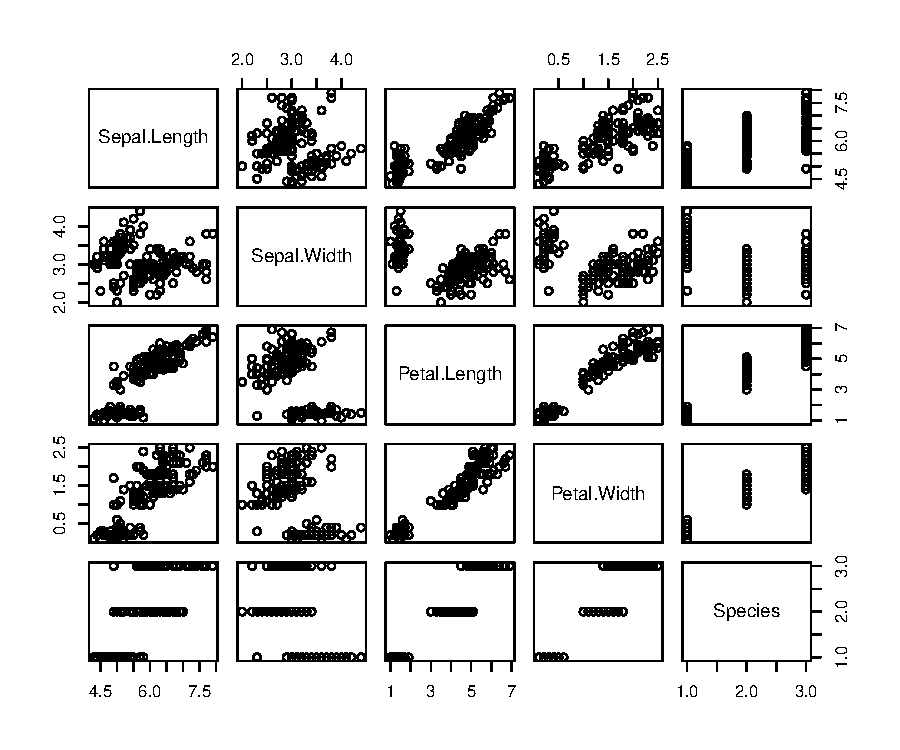
\includegraphics[width=\maxwidth]{plots/pplot-1} 

\end{knitrout}
\end{center}
\caption{Pairs plot for iris data.}
\label{fig:pairs}
\end{figure}

% =======================================
\section{Methods}\label{sec:methods}
% =======================================

\paragraph{Statistical Methods}

In this report we use \cite{R}. In what follows there is some
dummy text in latin.

Lorem ipsum dolor sit amet, consectetuer adipiscing elit. Ut purus
elit, vestibulum ut, placerat ac, adi- piscing vitae, felis. Curabitur
dictum gravida mauris. Nam arcu libero, nonummy eget, consectetuer
id, vulputate a, magna. Donec vehicula augue eu neque. Pellentesque
habitant morbi tristique senectus et netus et malesuada fames ac turpis
egestas. Mauris ut leo. Cras viverra metus rhoncus sem. Nulla et lectus
vestibulum urna fringilla ultrices. Phasellus eu tellus sit amet tortor
gravida placerat. Integer sapi- en est, iaculis in, pretium quis,
viverra ac, nunc. Praesent eget sem vel leo ultrices bibendum. Aenean
faucibus. Morbi dolor nulla, malesuada eu, pulvinar at, mollis ac,
nulla. Curabitur auctor semper nulla. Donec varius orci eget risus.
Duis nibh mi, congue eu, accumsan eleifend, sagittis quis, diam. Duis
eget orci sit amet orci dignissim rutrum. 

Nam dui ligula, fringilla a, euismod sodales, sollicitudin vel, wisi.
Morbi auctor lorem non justo. Nam lacus libero, pretium at, lobortis
vitae, ultricies et, tellus. Donec aliquet, tortor sed accumsan bibendum,
erat ligula aliquet magna, vitae ornare odio metus a mi. Morbi ac
orci et nisl hendrerit mollis. Sus- pendisse ut massa. Cras nec ante.
Pellentesque a nulla. Cum sociis natoque penatibus et magnis dis parturient
montes, nascetur ridiculus mus. Aliquam tincidunt urna. Nulla ullamcorper
vestibulum turpis. Pellentesque cursus luctus mauris. 

\paragraph{Software} All analysis was performed in the \prog{R} programming language \citep{R}.

% =======================================
\section{Analysis} \label{sec:analysis}
% =======================================
Nulla malesuada porttitor diam. Donec felis erat, congue non, volutpat
at, tincidunt tristique, libero. Vivamus viverra fermentum felis.
Donec nonummy pellentesque ante. Phasellus adipiscing semper elit.
Proin fermentum massa ac quam. Sed diam turpis, molestie vitae, placerat
a, molestie nec, leo. Maecenas lacinia. Nam ipsum ligula, eleifend
at, accumsan nec, suscipit a, ipsum. Morbi blandit ligula feugiat
magna. Nunc eleifend consequat lorem. Sed lacinia nulla vitae enim.
Pellentesque tincidunt purus vel magna. Integer non enim. Praesent
euismod nunc eu purus. Donec bibendum quam in tellus. Nullam cursus
pulvinar lectus. Donec et mi. Nam vulputate metus eu enim. Vestibulum
pellentesque felis eu massa.

Quisque ullamcorper placerat ipsum. Cras nibh. Morbi vel justo vitae
lacus tincidunt ultrices. Lorem ipsum dolor sit amet, consectetuer
adipiscing elit. In hac habitasse platea dictumst. Integer tempus
convallis augue. Etiam facilisis. Nunc elementum fermentum wisi. Aenean
placerat. Ut imperdiet, enim sed gravida sollicitudin, felis odio
placerat quam, ac pulvinar elit purus eget enim. Nunc vitae tortor.
Proin tempus nibh sit amet nisl. Vivamus quis tortor vitae risus porta
vehicula. 

Fusce mauris. Vestibulum luctus nibh at lectus. Sed bibendum, nulla
a faucibus semper, leo velit ultri- cies tellus, ac venenatis arcu
wisi vel nisl. Vestibulum diam. Aliquam pellentesque, augue quis sagittis
posuere, turpis lacus congue quam, in hendrerit risus eros eget felis.
Maecenas eget erat in sapien mattis porttitor. Vestibulum porttitor.
Nulla facilisi. Sed a turpis eu lacus commodo facilisis. Morbi fringil-
la, wisi in dignissim interdum, justo lectus sagittis dui, et vehicula
libero dui cursus dui. Mauris tempor ligula sed lacus. Duis cursus
enim ut augue. Cras ac magna. Cras nulla. Nulla egestas. Curabitur
a leo. Quisque egestas wisi eget nunc. Nam feugiat lacus vel est.
Curabitur consectetuer.

Suspendisse vel felis. Ut lorem lorem, interdum eu, tincidunt sit
amet, laoreet vitae, arcu. Aenean fau- cibus pede eu ante. Praesent
enim elit, rutrum at, molestie non, nonummy vel, nisl. Ut lectus eros,
malesuada sit amet, fermentum eu, sodales cursus, magna. Donec eu
purus. Quisque vehicula, urna sed ultricies auctor, pede lorem egestas
dui, et convallis elit erat sed nulla. Donec luctus. Curabitur et
nunc. Aliquam dolor odio, commodo pretium, ultricies non, pharetra
in, velit. Integer arcu est, nonummy in, fermentum faucibus, egestas
vel, odio. 

% latex table generated in R 3.2.1 by xtable 1.7-4 package
% Tue May 31 14:18:16 2016
\begin{table}[!h]
\centering
{\footnotesize
\begin{tabular}{rrrr}
  \hline
 & Coefficient & 95\% confidence interval & $p$-value \\ 
  \hline
Intercept & 2.17 & from 1.62 to 2.72 & $<$ 0.0001 \\ 
  Sepal.Width & 0.50 & from 0.33 to 0.67 & $<$ 0.0001 \\ 
  Petal.Length & 0.83 & from 0.69 to 0.96 & $<$ 0.0001 \\ 
  Petal.Width & -0.32 & from -0.61 to -0.02 & 0.039 \\ 
  Speciesversicolor & -0.72 & from -1.20 to -0.25 & 0.003 \\ 
  Speciesvirginica & -1.02 & from -1.68 to -0.36 & 0.003 \\ 
   \hline
\end{tabular}
}
\caption{Linear regression model choosing some columns.} 
\label{tab:regmod1}
\end{table}
% latex table generated in R 3.2.1 by xtable 1.7-4 package
% Tue May 31 14:18:16 2016
\begin{table}[!h]
\centering
{\footnotesize
\begin{tabular}{rrrr}
  \hline
 & Coefficient & 95\%-confidence interval & $p$-value \\ 
  \hline
Intercept & 6.53 & from 5.58 to 7.47 & $<$ 0.0001 \\ 
  Width Sepal & -0.22 & from -0.53 to 0.08 & 0.15 \\ 
   \hline
\end{tabular}
}
\caption{Linear regression model with adapted row names.} 
\label{tab:regmod2}
\end{table}


% latex table generated in R 3.2.1 by xtable 1.7-4 package
% Tue May 31 14:18:17 2016
\begin{table}[!ht]
\centering
{\footnotesize
\begin{tabular}{rcccc}
  \hline
Sepal.Length & Sepal.Width & Petal.Length & Petal.Width & Species \\ 
  \hline
5.10 & 3.50 & 1.40 & 0.20 & setosa \\ 
  4.90 & 3.00 & 1.40 & 0.20 & setosa \\ 
  4.70 & 3.20 & 1.30 & 0.20 & setosa \\ 
  4.60 & 3.10 & 1.50 & 0.20 & setosa \\ 
  5.00 & 3.60 & 1.40 & 0.20 & setosa \\ 
  5.40 & 3.90 & 1.70 & 0.40 & setosa \\ 
   \hline
\end{tabular}
}
\caption{First six records of the iris dataset.} 
\label{tbl:head}
\end{table}
% latex table generated in R 3.2.1 by xtable 1.7-4 package
% Tue May 31 14:18:17 2016
\begin{table}[!ht]
\centering
{\footnotesize
\begin{tabular}{r|cc}
  \hline Species & \multicolumn{2}{c}{Petal.Width < 1.5} \\ & FALSE & TRUE \\ 
  \hline
setosa &   0 &  50 \\ 
  versicolor &  15 &  35 \\ 
  virginica &  49 &   1 \\ 
   \hline
\end{tabular}
}
\caption{Contingency table for iris data.} 
\label{tbl:cont}
\end{table}


% =======================================
% \section{References} \label{sec:ref}
% =======================================
\nocite{R}

\bibliography{consulting}


\vfill

\footnotesize

{\bf \prog{R} version and packages used to generate this report:}

\prog{R} version: \textsf{R version 3.2.1 (2015-06-18)}

Base packages: \textsf{stats, graphics, grDevices, utils, datasets, methods, base}

Other packages: \textsf{lqmm, lme4, Matrix, dplyr, plyr, ggplot2, lattice, RColorBrewer, biostatUZH, survival, reporttools, xtable, knitr}

This document was generated on May 31, 2016 at 14:18.



\end{document}
